%\documentclass{acmsiggraph}               % final
%\documentclass[review]{acmsiggraph}      % review
%\documentclass[widereview]{acmsiggraph}  % wide-spaced review
\documentclass[preprint]{acmsiggraph}    % preprint

%% Uncomment one of the four lines above depending on where your paper is
%% in the conference process. ``review'' and ``widereview'' are for review
%% submission, ``preprint'' is for pre-publication, and ``final'' is for
%% the version to be printed.

%% These two line bring in essential packages: ``mathptmx'' for Type 1 
%% typefaces, and ``graphicx'' for inclusion of EPS figures.

\usepackage{mathptmx}
\usepackage{graphicx}

%% use this for zero \parindent and non-zero \parskip, intelligently.

\usepackage{parskip}

%% If you are submitting a paper to the annual conference, please replace 
%% the value ``0'' below with your OnlineID. If you are not submitting this
%% paper to the annual conference, you may safely leave it at ``0'' -- it 
%% will not be included in the output.

\onlineid{0}

%% need to document this!

\acmformat{print}

%% Paper title.

\title{Tangible User Interfaces... (TODO)}

%% Author and Affiliation (single author).

%%\author{Roy G. Biv\thanks{e-mail: roy.g.biv@aol.com}\\Allied Widgets Research}

%% Author and Affiliation (multiple authors).

\author{Christian Prossenitsch\thanks{e-mail: e0925433@student.tuwien.ac.at}\\ Vienna University of Technology %
\and Karin Pfattner\thanks{e-mail: insert email here}\\ Vienna University of Technology}%

%% Keywords that describe your work.

\keywords{radiosity, global illumination, constant time TODO}

%%%%%% START OF THE PAPER %%%%%%

\begin{document}

%% The ``\maketitle'' command must be the first command after the
%% ``\begin{document}'' command. It prepares and prints the title block.

\maketitle

%% Abstract section.

\begin{abstract}


In this paperl compare and analyze different Tangible User Interfaces. TUIs move away from the common input devices like mouse and keyboard and towards a direct interaction with physical objects in order to make the operation with devices more natural. This includes for example the handling of physical objects on tabletops, projections of information onto pieces of paper \cite{holman05} or using additional devices to get more detailed data. The examples we are going to cover in this paper include applications in architecture, information visualization and learning tools. 



\end{abstract}

%% ACM Computing Review (CR) categories. 
%% See <http://www.acm.org/class/1998/> for details.
%% The ``\CRcat'' command takes four arguments.

\begin{CRcatlist}
  \CRcat{K.6.1}{Management of Computing and Information Systems}%
{Project and People Management}{Life Cycle};
  \CRcat{K.7.m}{The Computing Profession}{Miscellaneous}{Ethics}
\end{CRcatlist}

%% The ``\keywordlist'' command prints out the keywords.
\keywordlist

\section{Introduction}

%% The ``\copyrightspace'' command must be the first command after the 
%% start of the first section of the body of your paper. It ensures the
%% copyright space is left at the bottom of the first column on the first
%% page of your paper.

\copyrightspace

Lorem ipsum dolor sit amet, consetetur sadipscing elitr, sed diam
nonumy eirmod tempor invidunt ut labore et dolore magna aliquyam erat,
sed diam voluptua. At vero eos et accusam et justo duo dolores et ea
rebum. Stet clita kasd gubergren, no sea takimata sanctus est Lorem
ipsum dolor sit amet. Lorem ipsum dolor sit amet, consetetur
sadipscing elitr, sed diam nonumy eirmod tempor invidunt ut labore et
dolore magna aliquyam erat, sed diam voluptua. At vero eos et accusam
et justo duo dolores et ea rebum. Stet clita kasd gubergren, no sea
takimata sanctus est Lorem ipsum dolor sit amet. Lorem ipsum dolor sit
amet, consetetur sadipscing elitr, sed diam nonumy eirmod tempor
invidunt ut labore et dolore magna aliquyam erat, sed diam
voluptua. At vero eos et accusam et justo duo dolores et ea
rebum. Stet clita kasd gubergren, no sea takimata sanctus est Lorem
ipsum dolor sit amet.

Duis autem vel eum iriure dolor in hendrerit in vulputate velit esse
molestie consequat, vel illum dolore eu feugiat nulla facilisis at
vero eros et accumsan et iusto odio dignissim qui blandit praesent
luptatum zzril delenit augue duis dolore te feugait nulla
facilisi. Lorem ipsum dolor sit amet, consectetuer adipiscing elit,
sed diam nonummy nibh euismod tincidunt ut laoreet dolore magna
aliquam erat volutpat.

Ut wisi enim ad minim veniam, quis nostrud exerci tation ullamcorper
suscipit lobortis nisl ut aliquip ex ea commodo consequat. Duis autem
vel eum iriure dolor in hendrerit in vulputate velit esse molestie
consequat, vel illum dolore eu feugiat nulla facilisis at vero eros et
accumsan et iusto odio dignissim qui blandit praesent luptatum zzril
delenit augue duis dolore te feugait nulla facilisi.
\section{Typical designs of Tangible User Interfaces}

In this section we will discuss different hardware implementations of tangible user interfaces and take a look on the different design spaces they are used in. 
The graphical user interface (GUI) with the input devices of mouse and keyboard falls short in embracing the rich interface modalities between people and the physical environment they inhabit \cite{ullmer97}. 

The interpretation of tangible user interfaces varies throughout the field. Ullmer and Ishii \cite{ullmer97} 

design spaces include bur are not limited to
- information visualization
- architectural
- geographical
- "entertainment"


we give first example of stationary display with fixed devices , then more free ones


\subsection{metaDESK}
One of the attemps in broadening the input possibilities to different devices is the metaDESK system introduced by Ullmer and Ishii \cite{ullmer97}. They describe a "Tangible User Interface" (TUI) as a user interface employing physical objects, instruments, surfaces, and spaces as physical interfaces to digital information. The metaDESK system consists of: a desk, a nearly-horizontal backprojected graphical surface; an active lens an arm-mounted flat-panel display; one or more passive lenses, an optically transparent surface through with the desk projects; and an assortment of physical objects an instruments which are used on the desk's surface. The components are sensed by an array of optical, mechanical and electromagnetic field sensors.

The focus lies on the use of real physical objects as driving elements of human-computer interaction. The approach of Ullmer and Ishii allthough tries to take elements of the GUI and bringing it into the real world as well as pushing forward from the unaugmented physical world, inheriting from vaious historical instruments and devices often "obsoleted" by the advent of the computer, like the active lens which is based on a jeweler's magnifying lens. The models for the objects are taken from everyday objects from home, scientific instruments or drawing and design tools. The material they used was transparent machined acrylic, designed to minimize occlusion of the desk surface.

The GUI icons are instantiated as "phicons" (physical icons), menus and handles are instantiated as TUI "trays" and "phandles" (physical handles), scales and scrollbars as TUI instruments such as a rotation constraint instrument. 

To test the system they implemented a prototype application called "Tangible Geospace" allowing interaction with geographical space.
The models themselves act as information containers about the object they represent as well as physical handles for manipulating the map.

The arm mounted active lens is coupled to the models and displays three-dimensional views of the scene and moving the lens makes it possible to navigate throu 3D space. This allows a seamless interaction with three spaces at once: the physical space of the object, the 2D graphical space of the desk's surface and the 3D graphical space of the active lens.

It is also possible to place a second object on the table, allowing the user to scale or rotate the map by moving the objects with respect to each other. This also allows collaboration as each object may be manipulated by an individual user. The sensing is performed by a computer-vision system inside the desk unit, along with magnetic -field position sensors and electrical contact sensors.

The passive lenses consist of a transparent surface that functions as an independent display when augmented by the back-projected desk. Since they are passive transparent surfaces, many vaiously afforded lenses might be used simultaneously with no additional active display resources.

As alternative to the two phicon scaling/rotation interaction, a rotation constraint instrument made of two cylinders mechanically coupled by a sliding bar might be used.
Albeit the extension of input methods it is not the goal of metaDESK to replace GUIs, but rather to complement them by providing new opportunities for human-computer interaction. 



\subsection{Other solutions to Tangible Interfaces}
Spindler, Tominski, Schuhmann and Dachselt \cite{spindler10} introduce 'tangible views' for use in Information Visualization as spatially aware lightweight displays that can be interacted with by moving them through the physical space on or above a tabletop surface. 

The motivation for their project is the difficulty of encoding all information in a single image once a data set exceeds a certain size or complexity. This problem can be solved spatially by providing multiple views on the data or embedding additional local views in the visualization or it can be solved temporally by changing the representations over time. They define a tangible view as a physical surface, that users can hold in their hands with no restrictions on size and shape.
 
Tangible views serve two purposes: It is used as a local display in conjunction with a tabletop display, and as an input device. The specific graphical information is projected onto the tangible view and three dimensional manipulation of a tangible view is tracked in space to make six degrees of freedom available: position (x, y, z) with respect to the interaction space and local orientation of the tangible view ($\alpha$, $\beta$, $\gamma$). It is also possible to use multiple tangible views at the same time. 

In summary tangible views:
\begin{itemize}
\item Integrate display an interaction device.
\item Enhance common 2D interaction with additional 3D interaction
\item Replace virtual views by physical, tangible views.
\end{itemize}

Tangible views do not exist on their own, but are integrated into an environment of one or more stationary displays of arbitrary size, shape and orientation. 
They also describe a basic display configuration consisting of a horizontal tabletop for the main context view and tangible views as local views into the information space. This relates to the focus and context concept.




\subsection{Including social aspects}
Hornecker and Buur \cite{hornecker06} extend the thought of tangible user interfaces further to 'tangible interactions'. They introduce a framework that focuses on the interweaving of the material/physical and the social, laying the ground for collaboration-sensitive tangible interaction design. It relies on tangibility and full-body interaction and gives computational resources and data material form, embedding computing in the everyday environment, digitally augmenting physical space and supporting intuitive use. 

Designing tangible interfaces requires not only designing the digital but also the physical, and their interrelationships within hybrid ensembles, as well as designing new types of interaction that can be characterized as full-body, haptic, and spatial.
Applications previously not considered interfaces are turning into such and computing is increasingly embedded in physical environments.

They distinguished three different views on tangible interfaces:
\begin{itemize}
\item Data-centered view: Here 'tangible interfaces' are understood as utilizing physical representation and manipulation of digital data, offering interactive couplings of ohysical artifacts with "computationally mediated digital information", Eg. Ullmer and Ishii
\item Expressive-Movement-centered view: Aiming to design interaction itself by emphasizing bodily interaction with objects, exploiting the "sensory richness and action potential of physical objects" so that "meaning is created in the interaction". <--!!quote!!
\item Space-centered view: 'Interactive spaces' as "Interactive systems, physically embedded within real spaces, offer opportunities for interacting with tangible devices" and so "trigger display of digital content or reactive behaviours" The body is used as interaction device and display.
\end{itemize}

Tangible interaction encompasses a broad range of systems and interfaces, building upon and synthesizing these views. These share the following characterisitcs: tangibility and materiality, physical embodiment of data, embodied interaction and bodily movement as an essential part of interaction, and embeddednes in real space, designing the interaction itself and exploiting the richness of bodily movement.

Their framework is structured around four interrelated themes:
\begin{itemize}
\item Tangible Manipulation:  material representations with distinct tactile qualities which are physically manipulated.
\item Spatial Interaction: tangible interaction is embedded in real space and therefore occurs by movement in space.
\item Embodied Facilitation: how the configuration of material objects and space affects and directs group behaviour.
\item Expressive Representation: material and digital representations employed ba tangible interaction systems, their expressiveness and legibility.
\end{itemize}




% Design and Hardware
\section{Examples of Tangible User Interfaces}
There is a wide variety of Tangible User Interfaces (TUIs). Possible applications for TUIs are literally endless. Many systems of TUIs have been explored and published in the past, but still a lot of new a ideas are coming up and new applications for TUIs are going to be explored. In this section, we will give examine some examples of TUIs and give an overview of different domains where TUIs have been successfully deployed.

\subsection{Table-top environments}
Many TUIs rely on table-top environments as their interaction technique. In these environments, a IR camera is set underneath the table-top to track fiducial markers placed onto the table. The camera can also track touch interactions of users. Marker and touch-based interactions are used as user input to the TUI system. The system responds to the user interactions by projecting visual feedback onto the table-top.

\subsubsection{reacTable}
The reactAble, presented by \cite{jorda07}, is a musical instrument based on a table-top TUI. Fiducial Markers represent musical objects, which generate sound according to their relation to each other. The markers are tracked by an IR camera. According to their attached symbol, each object has a dedicated function. The objects can be categorized in six different functional groups: audio generators, audio filters, controllers, control filters, mixers and global objects. \shortcite{jorda07}

ReacTIVision, the computer vision system behind reactAble, tracks the fiducial markers and sends the output data to an audio synthesizer. The waveforms generated by the synthesizer, as well as the data from the ReacTIVision tracker are sent to a visual synthesizer. The visual synthesizer projects visual feedback back onto the table-top. The audio lines that connect objects show the real resulting waveforms. Visual feedback is also used to monitor the objects state and internal parameters. Fingers can be used to either modify the objects parameters, or to cut (i.e. mute) audio connections between objects. \shortcite{jorda07}

\begin{figure}
\centering
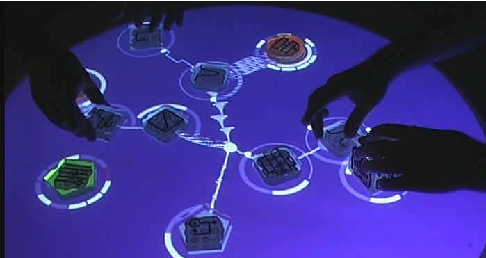
\includegraphics[width=0.45\textwidth]{figures/reactable.pdf}
\caption{The reacTable in action (compare \shortcite{jorda07})}
\label{fig:reactable}
\end{figure}
%TODO: reference figure!!

Modular synthesis is used for the sound generation process. Modular synthesis is based on the interconnection of sound generators and sound processor units. In reactAble, automatic connections between objects are made depending on the type of objects involved and the proximity between them. By moving objects around and bringing them into relation to each other, performers construct and play instruments at the same time. reactAble is also a collaborative tool for interactive live music. Because of the rather big size of the table-top, multiple artists can perform together on a single reacTable. \shortcite{jorda07}

\subsubsection{TARboard}
TARBoard is a tangible augmented reality system designed for table-top game environment. The purpose of TARboard is is to let users enjoy games in a more interactive and intuitive way and to make games more realistic and immersive. \shortcite{lee05}

Markers are attached to objects or cards used in a game. Similar to reactAble, these markers are tracked on a table-top environment by a camera underneath it. The augmenting camera is placed above the table-top. It provides the video stream for augmenting a game with virtual objects. \shortcite{lee05}

\cite{lee05} implemented a card game as a prototype for TARboard. Each player has cards which represent mystic creatures. The marker on the bottom of each card is tracked by the tracking camera. When the players flip a card and place it near the battle zone, the creatures get augmented on the battle zone and fight against each other.

\subsection{Urban planning workbenches}
In urban planning, designers usually employ three forms of representation: Two-dimensional drawings on sheets of papers, three-dimensional physical models and computer models, which can be two and three-dimensional. Each of these representations are created and displayed independently. Urban planning workbenches try to bridge the gap between these forms of representation, by simultaneously layering 2D drawings, 3D physical models, and digital simulation over each other. 
First, the 2D drawings and sketches are laid out on a table. Next, the 3D models are placed on top of the drawings. Finally, video projectors project digital simulations onto the surface. Video cameras capture the activity on the table and adjust the dynamic representation according to the position of the drawings and models with optical tags. \cite{ishii02}

\subsubsection{Urp}


\subsubsection{The Luminous Table}

\section{Tangible User Interfaces in Visualization}
The purpose of this chapter is to introduce Tangible User Interfaces which are settled in the domain of Visualization. We will give an overview of TUIs in Visualization we consider noteworthy. In the previous chapter, some of the presented TUIs could also be labeled as TUIs for Visualization, because some output is visualized by the system. In the reacTable for example, the sound waves between different musical objects are visualized on the tabletop. However, the reactAble is designed as a musical instrument. In this chapter, we will focus explicitly on TUIs, which sole purpose is the Visualization of data.

\section{Tangible Views for Information Visualization}
Tangible Views is a Tangible User Interface for Information Visualization presented by \cite{spindler10}. It consists of several handheld displays, which allow to interact with the visualized data in a more direct way. Similar to Paper Windows, a TUI presented by \cite{holman05}, the information is project onto cardboard displays (tangible views) as well as a tabletop. The setup also consists of several IR cameras, which track the tangible views and make them spatially aware. Gestures performed on the tangible view are recognized by the system as well. 

\section{discussion}
\section{Conclusion}
We have examined different designs of Tangible User Interfaces in this report. Furthermore, we have presented and discussed several examples of TUIs. Although the focus of this work lies in TUIs for visualization, we have also presented TUIs for other domains. A discussion about different aspects of TUIs followed their presentation. 

TUIs can be intuitive tools for the examination of visualized data. Instead of using the classic mouse and keyboard interaction, they enable users a more natural way of exploration and interaction with digital content. By using graspable objects and multi-touch gestures, users learn the interaction patterns more easily. This results in a faster and more comfortable way of examining visualized information. The TUI interaction paradigms work especially well for huge amount of data with multiple layers. However, TUIs are normally specialized on certain visualization tasks. Therefore, TUIs can only interact with certain styles of visualizations effectively. Everyday tasks like writing or navigating through documents or searching the web are still accomplished faster with traditional ways of computer interaction.

%should be on top of last page
\begin{figure}
\centering
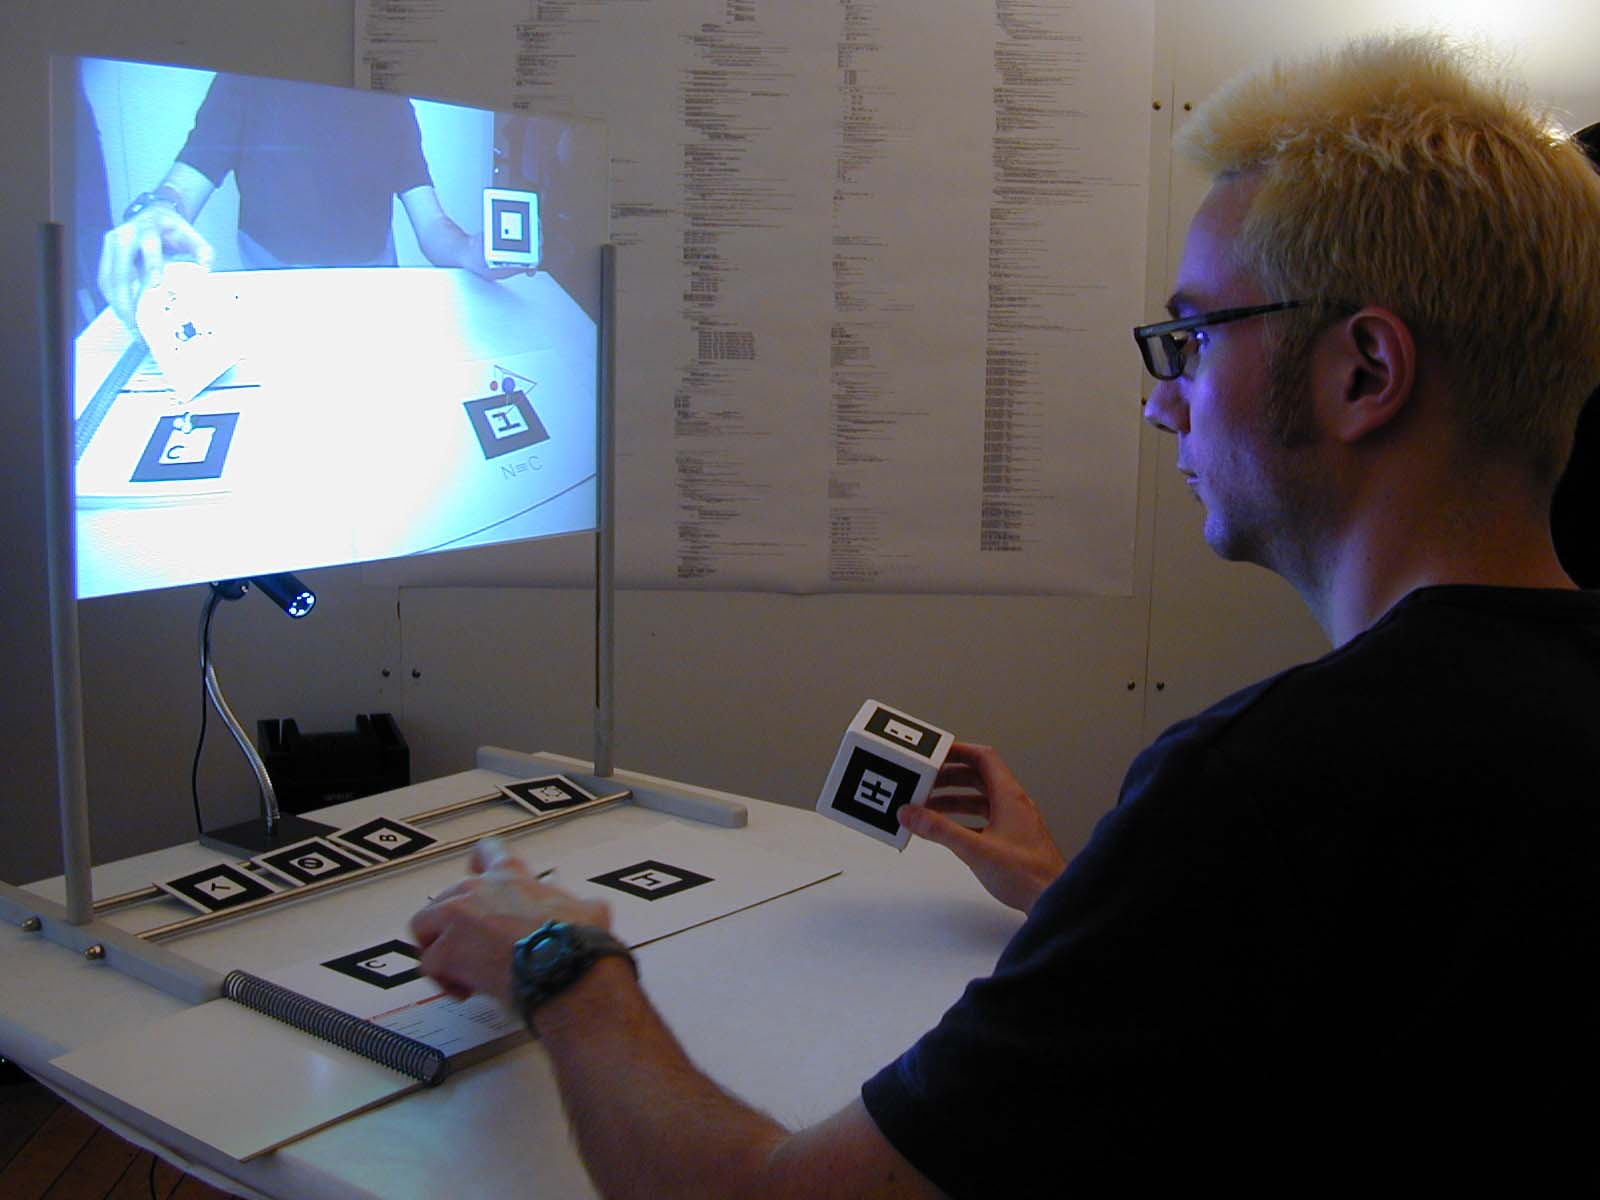
\includegraphics[width=0.47\textwidth]{figures/augmented_chemistry.jpg}
\caption{Augmented Chemistry in action (compare \protect\cite{fjeld02})}
\label{fig:augmented_chemistry}
\end{figure}

\bibliographystyle{acmsiggraph}
\nocite{*}
\bibliography{template}
\end{document}
